\chapter{NVM-enabled hash table} \label{OwnWork}
In this chapter we will discuss the key component of our system which allows us to reliably manage data locally using the non-volatile memory. 

\section{Overview}

    Each replica of \DHTS stores data locally in a purpose-built, NVM-enabled, generic hash table called \emph{\PersistentHashTable} (\PHT). \PHT exports an interface similar to Java's \HashMap \cite{HashMapJava}, and thus provides the following basic operations: \insertMethod, \getMethod or \removeMethod. Additionally, \PHT features iterators (through the \Iterator class), which can be used to perform scan operations over the entire data structure.
    
    When used with the \texttt{int} data type, \PHT relies on a deterministic hashing algorithm provided by John Lamping and Eric Veach \cite{Hashing}. On the other hand, in case one wants to use \PHT with non-standard, custom-defined data types, an additional hashing function has to be provided.
    
    In order to utilise the capabilities of the modern multicore CPU architecture, \PHT is implemented in a way that enables efficient concurrent access by multiple threads. 
    To this end we follow the design of \ConcurrentHashMap from Java 7 \cite{ConcurrentHashMapJava}. 
    In this approach, a hash table is composed of several smaller hash tables (which we call \internalHashMaps), each of which is guarded by a separate readers-writer lock and can expand independently from the other \internalHashMaps. 
    An \internalHashMap is simply an array of linked lists containing key-value pairs; all nodes in the same linked list share the hash of the nodes' keys.
    
    Since \PHT is built on top of NVM, its design and implementation differs significantly from the original hash table, which we used as an inspiration. 
    In particular, \PHT is implemented in a way, which allows it to cope with process crashes (due to, e.g., power outages) without compromising the consistency of the data. 
    To access NVM, we use the \libpmemobj library \cite{Libpmemobj}.
    
\section{Implementation}

    In Listing~\ref{NvmHashMap} we show the declaration of the \NvmHashMap template, which implements \PHT. Besides the basic hash table methods (\getMethod, \insertMethod, \removeMethod), the template features several other components:
    \begin{itemize}
        \item \texttt{loadFactor} -- a value which is used to determine when an \internalHashMap should be expanded in order to keep hash collisions low (situations in which multiple key-value pairs are mapped to the same hash); \texttt{loadFactor} can be adjusted upon object creation through the class constructor; the default value of \texttt{loadFactor} is 0.7, 
        \item \texttt{internalHashMap} -- an array of the \internalHashMap objects; its initial size is set to 8 and, similarly to \texttt{loadFactor}, can be adjusted through the class constructor (it is then rounded down to the largest power of 2 smaller or equal to the value provided by the programmer),
        \item \texttt{locks} -- an array of readers-writer locks; each lock is responsible for guarding accesses to a separate \internalHashMap.
    \end{itemize}

\begin{figure}[ht] 
\renewcommand{\figurename}{Listing}
    \begin{lstlisting}
template<class K, class V> 
class NvmHashMap {
    double loadFactor;
    int32_t hash(K key);
    pmem::obj::persistent_ptr <InternalHashMap<K,V>[]> internalHashMap;
    pmem::obj::persistent_ptr <pmem::obj::shared_mutex[]> locks;
    
    public: 
        NvmHashMap(double loadFactor);
        NvmHashMap(int threads);
        NvmHashMap(double loadFactor, int threads);
        V insert (K key, V value);
        V get (K key);
        V remove (K key);
        int size();
    
    friend class Iterator<K,V>;
}
    \end{lstlisting}
\caption{\NvmHashMap interface}
\label{NvmHashMap}
\end{figure}

    Below we discuss the most important aspects of \PHT's implementation.
    
\subsection{Support for generic types} 

    In \NvmHashMap each hash is of the type of \texttt{int32\_t}. 
    Since \NvmHashMap is a generic data structure, we must be able to calculate the hash value of keys of arbitrary types.
    For \texttt{int} data types we provide a hash method \cite{Hashing} presented in Listing~\ref{Hash}, for other basic types one must use a casting function. 
    
    \begin{figure}[ht]
\renewcommand{\figurename}{Listing}
\begin{lstlisting}
    int32_t hash(K key, int32_t range = 10000000) {
        int64_t key = key.convertToInteger(key);
        int64_t b = 1;
        int64_t j = 0;
        for (int i = 0; i < 5; i++) {
            b = j;
            key = key * 2862933555777941757ULL + j;
            j = (b + 1) * (double(1LL << 31) / double((key >> 33) + 1));
        }
        return fabs(b % range);
    }
\end{lstlisting}
\caption{The \texttt{hash} function.}
\label{Hash}
\end{figure}

    Using custom-defined data types with \NvmHashMap requires providing an additional method casting the data type to integer.
    To this end, the programmer needs to overload the comparison operator, which is used by \NvmHashMap to compare key-value pairs. 
    In Listing~\ref{StdHashOverload} we demonstrate how to define a custom casting method for a simple data structure \texttt{MyStruct}, which consists of two elements: \texttt{int} and \texttt{string}. 
    
    % To use custom-defined data types with \NvmHashMap, the programmer has to overload the comparison operator, used to compare key-value pairs, and provide a \texttt{to\_int} method which allows one to cast the object to an \texttt{integer}. 
    % In Listing~\ref{StdHashOverload} we demonstrate how to define a custom hash method for a simple data structure \texttt{MyStruct}, which consists of two elements: \texttt{int} and \texttt{string}. 
    
\begin{figure}[ht]
\renewcommand{\figurename}{Listing}
\begin{lstlisting}
struct MyStruct {
    int first;
    std::string second;
    
    bool operator==(const MyStruct &element) const {
        return (first == other.first && second == other.second);
    }
    
    int64_t convertToInteger(int first, std::string second) {
        int64_t result = 0;
        stringstream concatenated;
        concatenated << first << second;
        for(int i = 0; i < concatenated.length(); i++) {
            result += pow(concatenated[i], i);
        }
        return result;
    }
};
\end{lstlisting}
\caption{An example of a programmer-defined type usage}
\label{StdHashOverload}
\end{figure}

    During the development, at first we relied on the standard \texttt{hash} method from the \std namespace. It supported basic \std types and was efficient.
    However, we had to replace it once we realised, that --- following the documentation --- it was only \textit{required to produce the same result for the same input within a single execution of a program} \cite{StdHash}.
    Clearly, such guarantees were not enough for an application which uses NVM, because the data stored in this kind of memory may have been accessed repeatedly even after system shutdowns. In this case it is absolutely essential for the hash functor to provide the same result for the same key every time.    
    Therefore, we decided to use the described previously hashing algorithm.

\subsection{\internalHashMap}

    An \internalHashMap is a simple hash table built as an array of linked lists.
    We opted for this approach, because linked lists are supported out-of-the-box by \libpmemobj, the library for NVM which we use. 
    
    The basic element of \internalHashMap is called a \SegmentObject and it corresponds to a single key-value pair. \SegmentObject are arranged in linked list; all key-value pairs stored in the same linked list share a hash of their keys. A linked list which corresponds to a unique hash is called a \Segment (see Listing~\ref{Segment}). Each \Segment stores the hash value (the \texttt{hash} field) and the head of the list (the \texttt{head} field).

\begin{figure}[ht]
\renewcommand{\figurename}{Listing}
\begin{lstlisting}
class Segment {
    pmem::obj::p<int> hash;
    pmem::obj::persistent_ptr<SegmentObject<K, V>> head = nullptr;
}
\end{lstlisting}
\caption{Segment declaration.}
\label{Segment}
\end{figure}

    As we discuss later, operations on the linked list happen inside \pmdktransactions in order to preserve data consistency in case of a process crash.
    
    Each \internalHashMap object, whose declaration we show in Listing~\ref{internalHashMap}, is a collection of \Segment objects stored in an array. Initially, there are 16 \Segments in the \segments array. An \internalHashMap is a persistent object itself. We use the \texttt{elementsCount} field to store the number of elements in the entire \internalHashMap in order to be able to quickly obtain the size of the entire \NvmHashMap. We also use the value of \texttt{elementCount} to decide whether it is a proper time to resize \internalHashMap using the \expandMethod method.

\begin{figure}[ht]
\renewcommand{\figurename}{Listing}
\begin{lstlisting}
class internalHashMap {
    pmem::obj::persistent_ptr<Segment<K, V>[]> segments;
    pmem::obj::p<int> segmentsSize;
    pmem::obj::p<int> elementsCount;
    
    void expand();
}
\end{lstlisting}
\caption{\internalHashMap declaration.}
\label{internalHashMap}
\end{figure}

    In order for the \internalHashMap to resize, the \texttt{elementsCount} has to exceed the product of \texttt{arraySize} and \texttt{loadFactor} (which is by default set to 0.7, as in the original Java \HashMap \cite{HashMapJava}).
    Typically, we want \texttt{arraySize} to exceed \texttt{elementsCount} by some margin. Otherwise, there is a high probability that multiple key-value pair are stored in the same \Segment. Then, finding any of such pairs takes more time, as it requires iterating over the linked list inside \Segment. \texttt{arraySize} cannot be too large compared to \texttt{elementsCount}, because then we use a lot of memory to store few entries in the hash table.

    The \expandMethod method can be triggered only by the \insertMethod method. Once \expandMethod is called, we allocate a segment of persistent memory that is 4 times bigger than the one we used for the current \internalHashMap. Then, we iterate through the old \internalHashMap in order to insert all previously added elements to the new one. For each key-value pair we calculate a new hash. Note that the resizing of \internalHashMap happens independently for all \internalHashMap in \NvmHashMap.

\subsection{Concurrency} 
    
    The data integrity during concurrent access is provided by readers-writer locks (kept in the \locks array). More precisely, upon every access to an \internalHashMap, a corresponding lock is acquired either in the shared (\getMethod) or the exclusive mode (\insertMethod, \removeMethod). That way a thread performing an operation on \PHT does not prevent other threads from accessing different sections of \PHT at the same time. The number of sections (the size of the \internalHashMap array) should correspond to the expected number of concurrent threads accessing \PHT and the number of the available CPU cores. Note that resizing an \internalHashMap happens only as a result of a new key-value pair being inserted. Hence, the resizing operation happens when the appropriate lock is acquired in the exclusive mode, thus protecting the data from incorrect concurrent accesses by other threads.
            
    We use readers-writer locks instead of mutexes for performance reasons. This way several threads performing \getMethod operations can access simultaneously the same \internalHashMap. Naturally, \insertMethod and \removeMethod methods require exclusive access to \internalHashMap. Using readers-writer locks and an adjustable size of the \internalHashMap array means that \PHT \emph{supports full concurrency of retrievals and adjustable expected concurrency for updates} \cite{ConcurrentHashMapJava}. 
    
    Furthermore, as the \NvmHashMap provides an \Iterator, it is worth noting that ensuring a correct iteration over such a concurrent data structure is not easy. The \iterateMethod method uses only locks in the shared mode and therefore it may provide slightly inconsistent image of the hashmap while working in a multithreaded mode: the observed values might not correspond to a snapshot view of the hash table from any moment in time. If one thread starts iterating and another one removes an item afterwards, the first one may still see it in a hashmap. The same way, if one adds an element, it may not be visible for the second one yet. This inconsistency could have been solved using an exclusive mode of locking, albeit at the cost of reducing the availability of the data. Since \PHT is meant for a multithreaded environment, we prioritise low latency in data access.

\subsection{Operations on NVM}

    In order to correctly write to NVM, all write operations need to be carried out in \pmdktransactions, which guarantee that writes will be performed atomically. 
    This way the data stays consistent even in the event of possible system failures: when a crash occurs during execution of a transaction, the transaction is rolled back upon the application restart. Using PMDK transactions and locks allows us to safely and correctly access and modify data in NVM.

\begin{figure}[ht]
\renewcommand{\figurename}{Listing}
\begin{lstlisting}
V insert (K key, V value) {
    int hashMapIndex = chooseInternalHashMap();
    lock_exclusive(locks[hashMapIndex]);
    if (internalHashMap[hashMapIndex].elementsCount > 
            0.7 * internalHashMap[hashMapIndex].arraySize) {
        expand(hashMapIndex);
    }
    int result = insertIntoInternalHashMap
            (key, value, internalHashMap[hashMapIndex]);
    internalHashMap[hashMapIndex].elementsCount += result;
    unlock_exclusive(locks[hashMapIndex]);
}
    
int insertIntoInternalHashMap
        (K key, V value, internalHashMap<K, V> &aos) {
    int segmentIndex = chooseSegment();
    persistent_ptr element = aos.segments[segmentIndex].head;
    while (element->next) {
        if (element.key == key) {
            element.value = value;
            return 1;
        } 
        element = element -> next;
    }
    pmem::obj::transaction::run {
        element->next = 
                pmem::obj::make_persistent<SegmentObject <K, V>>();
        element->next->key = key;
        element->next->value = value;
        return 1;
    }
    return 0;
}
\end{lstlisting}
\renewcommand{\figurename}{Listing}
\caption{\insertMethod method}
\label{insertMethod}
\end{figure}
    
    We demonstrate how to access NVM using PMDK by showing the code of the \insertMethod method in Listing~\ref{insertMethod}. In order to insert a  key-value pair firstly we need to calculate two indexes. The first one, computed by the \texttt{choose\-Internal\-HashMap} method, indicates the appropriate \internalHashMap to use, whereas the second one, obtained using the \texttt{choose\-Segment} method, allows us to find the correct \Segment in the \internalHashMap. Both indexes are computed by hashing the key and performing bit operations to calculate the correct offset. Note that we obtain a lock of the appropriate \internalHashMap before calculating the second index. 
    
    Before a new key-value pair can be added to the \Segment, we check whether the expand function should be executed. If so, the \internalHashMap is resized and rehashed. 
    
    To insert a key-value pair, we iterate through the \Segment. If we find an element on the linked list (stored within the \Segment) with the same key, we update the value in a PMDK transaction. Otherwise, we also execute a PMDK transaction, in which the a new \SegmentObject containing the key and value is appended to the end of the list. Then we increment the value of \texttt{elementsCount}. Appending the \SegmentObject to the list as well as incremening \texttt{elementsCount} must be carried out in a transaction. Otherwise it is possible that upon process crash, the SegmentObject might be added to the list but \texttt{elementsCount} will stay unchanged thus making the data stored in \internalHashMap inconsistent.
        
\begin{figure}[ht]
\renewcommand{\figurename}{Listing}
\begin{lstlisting}
V get (K key) {
    int hashMapIndex = chooseInternalHashMap();
    lock_shared(locks[hashMapIndex]);
    int segmentIndex = chooseSegment();
    persistent_ptr element = internalHashMap[hashMapIndex].
                                    segments[segmentIndex].head;
    while (element->next) {
        if (element.key == key) {
            return element;
        }
        element = element -> next;
    }
    unlock_shared(locks[hashMapIndex]);
    throw "Did not found element" exception
}
\end{lstlisting}
\caption{\getMethod method}
\label{getMethod}
\end{figure}

        Since the \getMethod method does not modify any data, it does not need to run a PMDK transaction. Consequently, we can access data stored inside \internalHashMap in a straightforward way (see Listing~\ref{getMethod}). Note that in order to perform the \getMethod method, we obtain the appropriate lock in the shared mode. Using locks for read operations is necessary, because PMDK transactions do not provide any isolation guarantees, in particular to non-transactional code. It means that reading data stored in NVM (in or outside a transaction) could return corrupted data when there is a concurrent transaction that writes to the same memory locations. 

        
\begin{figure}[ht]
\renewcommand{\figurename}{Listing}
\begin{lstlisting}
V remove (K key) {
    int index = chooseInternalHashMap();
    lock_exclusive(locks[hashMapIndex]);
    int segmentIndex = chooseSegment();
    persistent_ptr element = internalHashMap[hashMapIndex].
        segments[segmentIndex].head;
    while (element->next) {
        if (element->next.key == key) {
            persistent_ptr temp = element->next->next;
            pmem::obj::transaction::run {
                element->next = temp;
                pmem::obj::delete_persistent(element->next);
                internalHashMap[hashMapIndex].elementsCount -= 1;
                return value;
            }
        }
        element = element -> next;
    } 
    unlock_exclusive(locks[index]);
    throw "Did not found element" exception
}
\end{lstlisting}
\caption{\removeMethod method}
\label{removeMethod}
\end{figure}

        The \removeMethod function (shown in the Listing~\ref{removeMethod}) is somewhat similar to the \insertMethod one. We first calculate the indexes for \internalHashMap and \Segment, acquire a lock in the exclusive mode and iterate over the \Segment. Finally, once a key to be deleted is found, we open a PMDK transaction and remove the corresponding \SegmentObject from the list and decrement \texttt{elementsCount}. If the element is not found, an exception is thrown.

\section{Evaluation}

\subsection{Correctness tests}
 
    In order to ensure that \PHT has been correctly implemented, we developed a range of unit tests. To this end we used the \GoogleTest library \cite{GoogleTest}. 
    We test our implementation for two different instances of the hashtable: \integersMap and \stringsMap.
    
    There are several tests performed.
    \begin{itemize}
    \item The first test works in single-threaded mode and inserts a number of elements with a known sum. 
        Then it iterates through \PHT and sums the elements up. 
        At the end an assert checks whether the two values are equal. 
        The test is run on both instances of \PHT, but in case of \NvmHashMap\stringsMap integers are cast to string.
    \item The next test focuses on the \getMethod method.
        We run it both in the single and the multithreaded mode (using 8 threads). 
        Each thread inserts 100,000 elements. 
        Then, the previously added values are retrieved. 
        In order for the test to complete successfully, all inserted items must be found. 
        Since the \getMethod method returns a value of the retrieved element, the obtained value is compared with the added one using an assert.
    \item The last test verifies the \removeMethod operation. 
        It is performed in two modes: single and multithreaded with 8 threads. 
        As in the previous test case, each thread inserts 100,000 elements. 
        Once they are inserted, the program tries to remove them from the \PHT. 
        Considering that the \removeMethod method returns the value of the deleted element, an assert checks for the equality of the obtained value and the added one. 
        The test ends as a success if all added values are removed.
    \end{itemize}

    One of issues that needs to be taken into account while developing unit tests is the non-volatile nature of the data kept in the \NvmHashMap. In a traditional system which uses traditional RAM, many tests can be performed in one test suite as the data kept in memory are automatically freed in-between tests. However, due to the use of NVM, \PHT keeps the data in the non-volatile memory even after a test completes. Therefore we need to manually manage memory in our test suites. To this end, we run each each test as a separate program instance. That way the files on which we operate to emulate NVM can be deleted and the memory cleared in between tests.  

    Developing the unit tests suite allowed us to find several bugs and therefore improve our implementation. One of encountered problems concerned the \Iterator class. If no item had been added to the \PHT, using \Iterator resulted in a program crash. Moreover, the preliminary test results made us look closer at the performance of the \insertMethod method, which took much longer to complete than expected. After a thorough analysis we were able to identify the \expandMethod method (triggered by \insertMethod) as a bottle neck.

    In order to check the data consistency of our system, we carried out several recovery tests, which proceeded as follows. First, we start a thread that is supposed to insert 1,000,000 elements to \PHT. Then we terminate the thread before it completes its work. Next, using an \Iterator we check what values were added to the \PHT and whether the application crashed. Once the application is operational, we insert the rest of the elements and ensure that all of them were added. Thanks to the use of PMDK transactions, we managed to ensure data consistency in all of our tests.
    
\subsection{Performance tests}

    % \tk{Can you increase the font size on the plots?}

    The performance tests aimed at comparing the effectiveness of the NVM-enabled \PHT with an analogous hash table, called \StandardHashMap, implemented in a traditional fashion, on top of RAM. \StandardHashMap provides the same interface as \NvmHashMap.
    
    The tests measured the time it takes to insert, get and remove 5,000,000 elements to the data structure. The number of items we insert into the hash tables is limited by the memory size. We conducted tests using the following environment:
    \begin{itemize}
        \item 8-core processor Intel Core i7-4720HQ CPU@2.6GHz, 0.8 GHz -- 3.6 GHz,
        \item RAM: 16 GB,
        \item RAM for NVM emulation: 4 GB,
        \item Operating system: Fedora Linux 27
    \end{itemize}
    We tested the data structures using 1, 2, 4 and 8 concurrent threads. 
    
    \begin{figure}[ht]
        \centering
        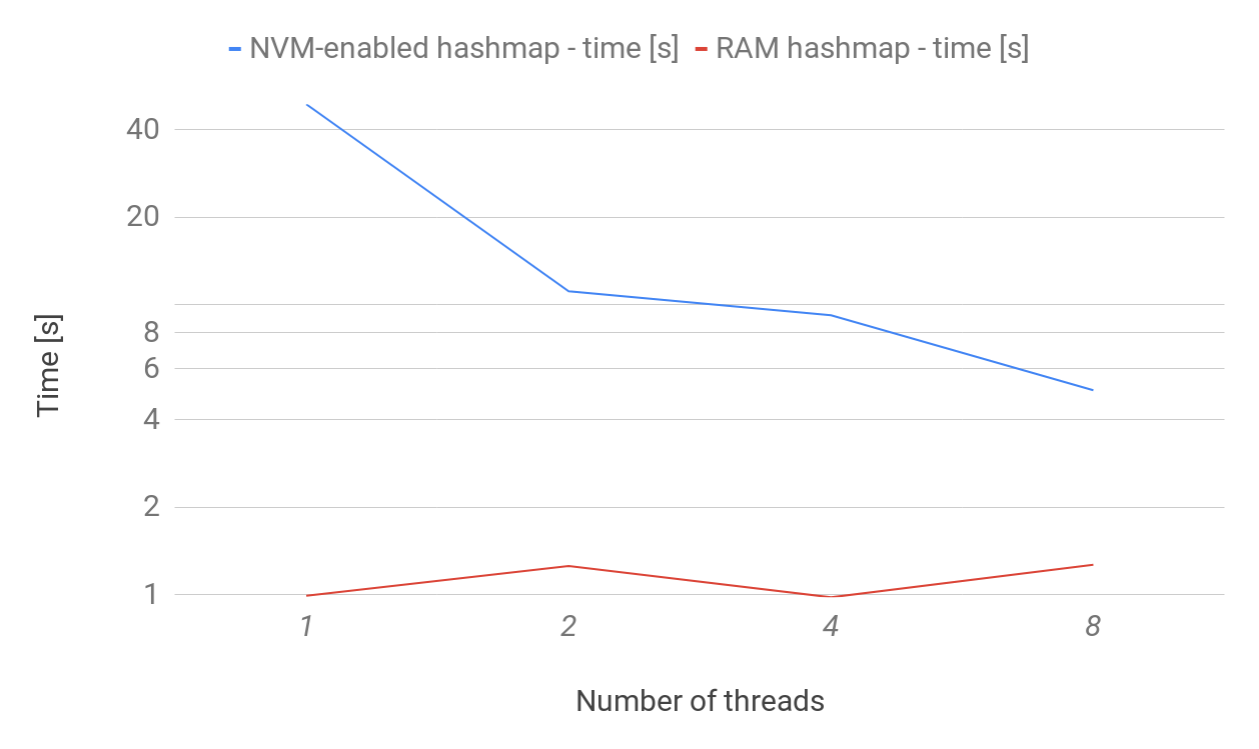
\includegraphics[width=0.8\textwidth]{thesis/figures/insert.png}
        \caption{Time necessary to perform 5,000,000 \insertMethod operations on \PHT and \StandardHashMap.}
        \label{insertPlot}
    \end{figure}
    
    \begin{figure}[ht]
        \centering
        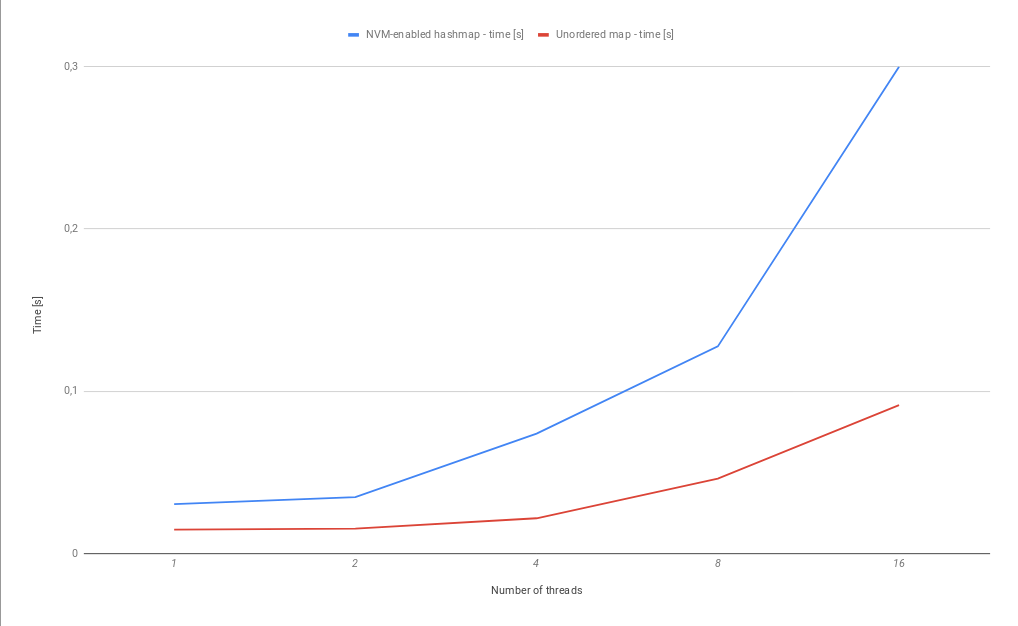
\includegraphics[width=0.8\textwidth]{thesis/figures/get.png}
        \caption{Time necessary to perform 5,000,000 \getMethod operations on \PHT and \StandardHashMap.}
        \label{getPlot}
    \end{figure}
    
    \begin{figure}[ht]
        \centering
        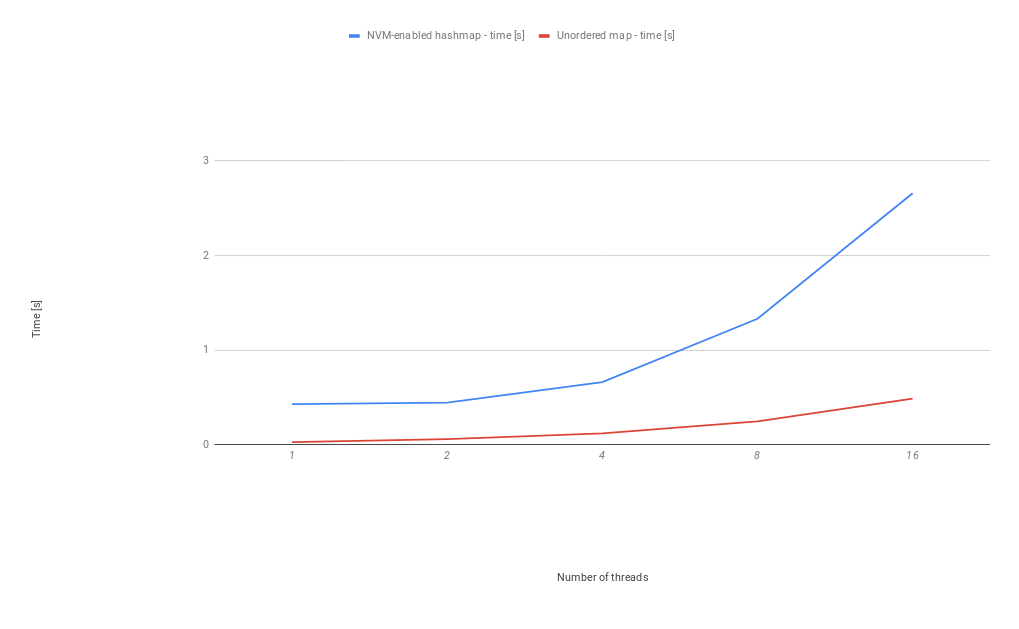
\includegraphics[width=0.8\textwidth]{thesis/figures/remove.png}
        \caption{Time necessary to perform 5,000,000 \removeMethod operations on \PHT and \StandardHashMap.}
        \label{removePlot}
    \end{figure}
    
    The tests results are shown on plots in Figures~\ref{insertPlot},~\ref{getPlot} and~\ref{removePlot}. One can see that in all test cases there is a noticeable NVM-induced time overhead. However, both our implementations scales well with the increasing number of threads.
    
    The \insertMethod method in the NVM implementation takes the longest time since it allocates memory and creates a new object. Furthermore, it requires an exclusive access to the \internalHashMap and resizes it when necessary. Since in each test the \texttt{threads} number varies, there is a different number of \internalHashMap objects. In the test with only one thread, the sole \internalHashMap expands about nine times while inserting 5,000,000 key-value pairs. On the contrary, the test with 8 threads uses 8 \internalHashMaps and therefore each of them expands 7 times on average. 
    
    The \getMethod operation is the fastest of implemented methods as it requires only a shared access to the \internalHashMap. It is about 2.5 times slower in the NVM-enabled implementation compared to \StandardHashMap, because \tk{what transaction in \getMethod? Not consistent with what you said earlier about the \getMethod method.} every time a transaction starts, PMDK creates a snapshot of the persistent memory.
    It is used for tracking the changes made during the transaction and may be used to revert them in case that the transaction will be rolled back.
    
    The \removeMethod method turns out to be about 5 times slower in the NVM-based environment than the RAM one. It turns out to be a little bit faster compared to the \insertMethod, because freeing an object requires less work compared to allocating memory. Still, however, \removeMethod needs to do so in a PMDK transaction. 
    
    Besides measuring the throughput of \PHT in comparison to the \StandardHashMap's performance, we are interested in the memory overhead resulting from storing data in NVM. \tk{In how much space?} In case of \StandardHashMap we are able to insert around 800,000 pairs \tk{what was in them, ints? strings? how big?} of \integersMap into the map. \PHT is less memory efficient and allows us to insert only 136,000 pairs of \integersMap. This disparity can be explained by the fact that currently the \libpmemobjcpp library allows one only to allocate pointers to persistent memory for blocks which are at least 4 KB in size.
    %\noindent \tk{What about the memory footprint? How many key-value pairs can you insert into lets say 100MB of memory in \PHT and \unorderedMap?}. 
    
    To sum up, \PHT is a considerably slower compared to \StandardHashMap, but it allows data to be recovered upon the process crash. The observed overhead is due to additional processing required when working with NVM. 
    %\tk{maybe something like: all operations on the persistent objects are performed within transactions which means that accessing each object requires writes to the internal PMDK log? this should be explained in Section 3.2.4 }. % described above 
    However, both implementations scale similarly well. 
            
\section{Conclusions}
        
    In this chapter we discussed \PHT, a custom-built hash table, which supports non-volatile memory. 
    % Implementing it meant overcoming a number of challenges, e.g. correctly defining operations within \tk{pmdk?} transactions, handling generic data types in and concurrency or choosing the suitable hash function. 
    % \tk{This kind of sentence probably should be in the final conclusions.} However, using the \libpmemobj library has helped us to understand better how NVM works. 
    Extensive tests allowed us to ensure its correctness and uncover several subtle bugs related to ensuring consistency of data upon process crashes.
    
    Unsurprisingly, \PHT turns out to be slower than a standard concurrent implementation of a hash table (\StandardHashMap), which relies solely on RAM. Our tests indicate that using NVM incurrs a significant but still acceptable overhead.
    The \getMethod method takes about 2,5 times more time to complete compared to its corresponding operation of the standard hash table, while \insertMethod and \removeMethod methods about 5-10 times on average. \PHT also requires around five times more memory compared to its traditional counterpart. \PHT handles well workloads in which there are multiple threads accessing it at the same time. \PHT's scalability is on par with the scalability of the standard hash table implementation.
    
